\documentclass{standalone}
\usepackage{tikz}

%% This version scales the whole diagram to one unit (1cm). Should be able to scale the entire drawing.

\begin{document}

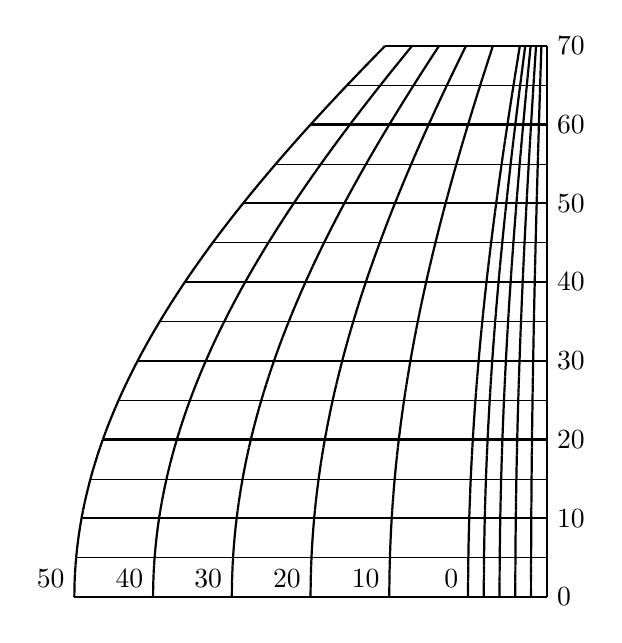
\begin{tikzpicture}[scale=10]
  %% \draw[blue,very thin, step=0.1cm] (-1,0) grid (0,1);
  \foreach \step in {0.00,0.02,0.04,0.06,0.08,0.1,0.2,0.3,0.4,0.5,0.6} { %for each of the curved lines
    \foreach \y in {0.0,0.01,...,0.69} {   %for each degree in the vertical scale
      \draw[thick]  ({(-sin(90-\y*100))*\step},\y) -- ({(-sin(90-(\y+0.01)*100))*\step},\y+0.01);
    }
  }
  \foreach \lat in {0, 10,...,70} {  %For each of the horizontal latitude lines
    \draw[thick] ({-sin(90-\lat)*.6},\lat/100) -- (0,\lat/100) node [right] {\lat};
  }
  
  \foreach \lat in {5,15,...,65} {  %For each of the thinner horizontal latitude lines
    \draw[very thin] ({-sin(90-\lat)*.6}, \lat/100) -- (0,\lat/100);
  }
  \foreach \min in {0,10,...,50} {     %For each minute in the latitude scale
    \node [above left] at (-\min/100-0.1, 0) {\min};
  }
\end{tikzpicture}

\end{document}
